\section{Limitations}
\begin{table}[htbp]
  \centering
  \caption{Overview of capacitive proximity sensing limitations}
    \begin{tabular}{p{4cm}p{6cm}}
    \toprule
    \textbf{Name} & \textbf{Examples} \\
    \midrule
    \textbf{Environmental influence} & Static electric fields, dynamic electric fields, temperature, humidity, conductive objects \\
    \textbf{Physical range} & Small differences in capacitance, reduction due to influences, physical limitations \\
    \textbf{Object detection} & Small number of data points, a priori knowledge \\
    \bottomrule
    \end{tabular}%
  \label{tab:cap_limitations}%
\end{table}%

Despite the potential that has been described in the previous sections there are various limitations of capacitive proximity sensing that we can put into the different groups of environmental influence, physical range and object detection that will be described in more detail in the following section. A short overview is given in Table \ref{tab:cap_limitations}.
\subsection{Environmental Influence}
One of the main limitations of capacitive proximity sensors is their sensitivity towards environmental influences. Any factor that modifies an electric field will also affect the measurement of a capacitive sensor. The current environmental parameters, like temperature and humidity are having a considerable effect on the atmosphere in which the electric field propagates. However, those changes are usually over a longer period of time and can be compensated using a factor for drift, as described in the previous sections about noise reduction. A more challenging factor is the other electric devices in the environment that emit stronger electromagnetic fields. While persistent sources, such as permanent electric installations can usually be countered using a galvanic isolation there are other non-obvious challenges. E.g. we noticed that certain plasma TVs are able to disturb the measurement and increase noise levels consider-ably. This change is even varying according to screen content. A minor effect is the presence of high-frequency fields that are getting more prevalent in modern IT equipped environments. Instead of the 2.4GHz and 5GHz ranges that are often used in wire-less communication, capacitive proximity sensors can operate in the range of a few kHz to one MHz. 
An additional issue might arise when placing sensors close to each other. The created electric fields may disturb the measurement if some electrodes are charged and create fields to adjacent electrodes while they are discharged for measurement. Consequently, specific charge-discharge cycles or multiplexing methods have to be used to counter this effect. 
A major challenge is dealing with conductive objects that are permanently placed in the immediate sensing environment. It is difficult to distinguish the object we want to detect from a disturbing object, if their influence on the electric field is similar. Long term data analysis may help in performing a successful detection.
The CapFloor prototype is affected by environmental influences the most, given the small size of the electrodes relative to the interaction area and the changing environment on top of the floor. We are using a strong noise reduction algorithm and drift compensation to create a more stable result while reducing the detection range.
\subsection{Physical Range}
\begin{figure}[h]
\centering
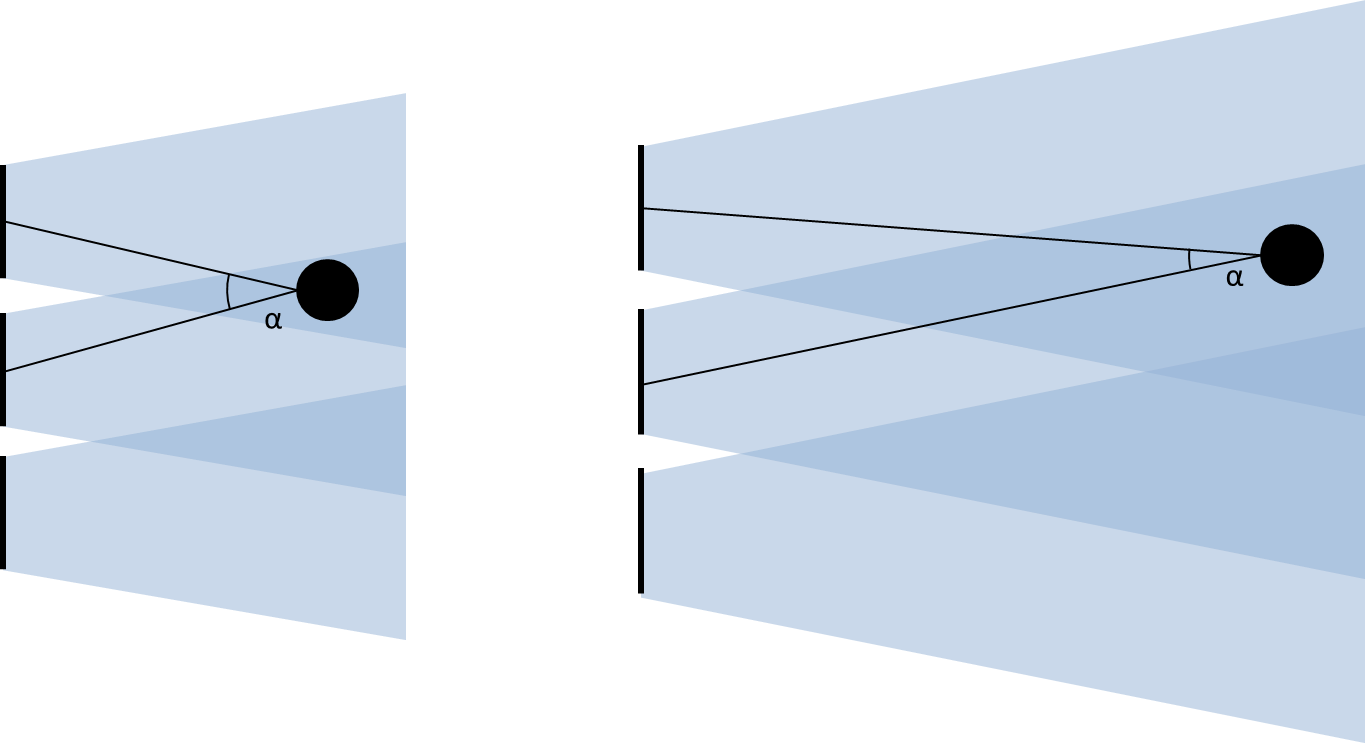
\includegraphics[width=0.6\textwidth]{images/limit_distance.png}
\caption{Reduced angular resolution on smaller, distant objects}
\label{fig:disc_ang_resolution}
\end{figure}
The physical range of the generated electric field is one of the main limiting factors of capacitive proximity sensing. In order to detect objects that are further away we have to increase the electric field strength sufficiently. This is easier the larger the electrode is, as its potential capacitance is higher. However, this also leads to distant objects having an ever smaller influence on the overall capacitance, and we need more precise measurement circuits and longer measurement times to improve the signal-to-noise ratio. Additionally, looking at smaller objects the angular resolution will decrease as shown in Figure \ref{fig:disc_ang_resolution}. This makes it more difficult to get a precise localization as the immanent noise leads to an angular error. While this can be compensated using more sensors, the far distance would require us to use large electrodes that have to be placed further apart resulting in a huge area that would have to be equipped with sensor electrodes.
In general the achievable resolution is not comparable to vision based system and has to be taken into consideration when designing the specific application. A balance between electrode size, physical range and achievable resolution has to be found.
The MagicBox size does not allow an integration of very large electrodes. Instead we are optimizing the available space in order to achieve a detection that lets us detect hands in a distance between 15 and 20 centimeters.
\subsection{Object Detection}
\begin{figure}[h]
\centering
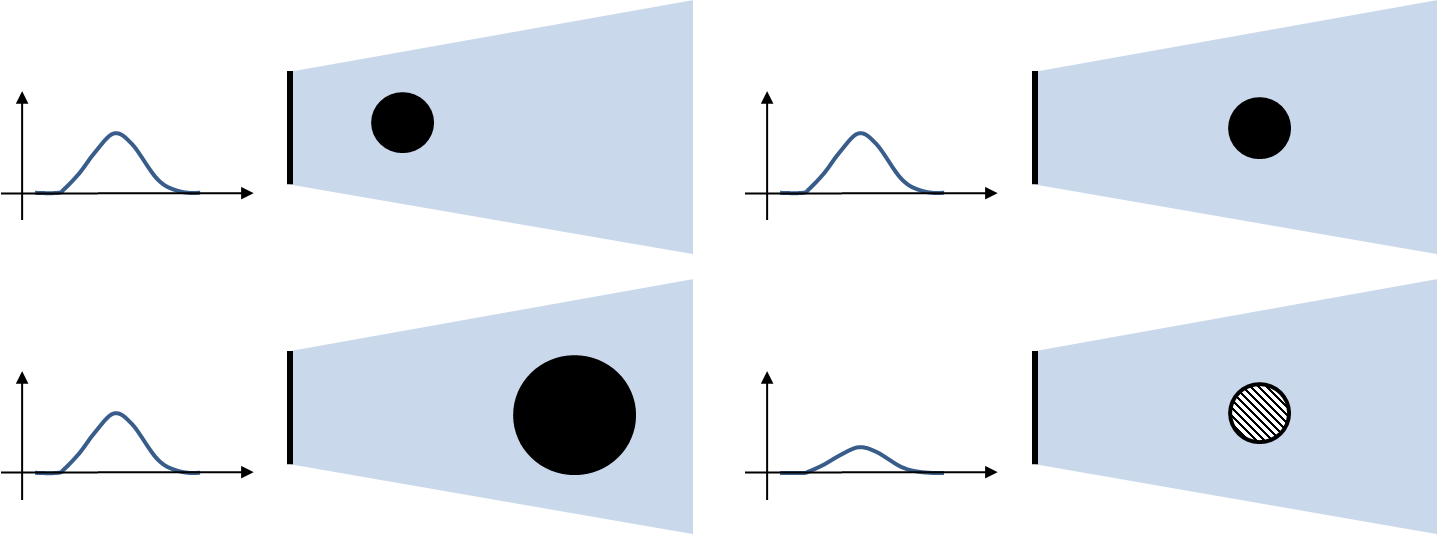
\includegraphics[width=0.6\textwidth]{images/limit_detection.png}
\caption{Same response to differently sized objects (left), different response to varying materials (right)}
\label{fig:disc_obj_detection}
\end{figure}
Object detection using capacitive sensors can be partially compared to object detection using camera systems, with a single sensor being equivalent to a single photo sensor. The light intensity measure is comparable to field intensity and likewise we can't distinguish if the measurement is caused by a weak source in close proximity or a strong source at a further distance. As a practical example the capacitive sensor can't decide if one hand is close to the sensor or two hands are a bit further away. This effect makes it challenging to provide object detection and we usually have to combine the information from various sensors to get a good idea about object shape and size. Due to the presented challenges in physical range and electrode size, capacitive proximity sensing systems do not have the same level of scalability as opposed to cameras, where millions of photo sensors can be placed in very small areas. 
Additionally, the effect of an object on the electric field is not always closely correlated to the object dimensions, but instead based on conductivity, material and other factors. We may get the same response to different objects at different distances or get a varying on similarly sized objects made of different materials, as shown in Figure \ref{fig:disc_obj_detection}. 
The Active Armrest has gestures for one and two fingers that are distinguished using a simple threshold. If another object is entering the field or the person has larger fingers the system will fail to properly differentiate gestures. Accordingly some other compensation methods should be used.

